%%%%%%%%%%%%%%%%%%%%%%%%%%%%%%%%%%%%%%%%%%%%%%%%%%%%%%%%%%%%%%%%%%%%%%%%%%%%%%%%%%%%
% Document data
%%%%%%%%%%%%%%%%%%%%%%%%%%%%%%%%%%%%%%%%%%%%%%%%%%%%%%%%%%%%%%%%%%%%%%%%%%%%%%%%%%%%
\documentclass[12pt]{article} %report allows for chapters
%%%%%%%%%%%%%%%%%%%%%%%%%%%%%%%%%%%%%%%%%%%%%%%%%%%%%%%%%%%%%%%%%%%%%%%%%%%%%%%%%%%%
\usepackage{preamble}

\begin{document}

\begin{center}
   \textsc{\large MATH 271, Homework 3, \emph{Solutions}}\\
   \textsc{Due September 20$^\textrm{th}$}
\end{center}
\vspace{.5cm}

\begin{problem}
Consider the second order chemical reaction given by
\[
A+B \xrightarrow{k} \textrm{Products}.
\]
\begin{enumerate}[(a)]
    \item Write a \emph{system} of differential equations to describe the concentration of the reactants $A$ and $B$ (this means write one for each).
    \item The concentrations of $A$ and $B$ can be related to each other in the following way: Let $A=A_0-x$ and $B=B_0-x$. Here, we think of $x$ as the amount of each chemical that has reacted, and note that it depends on time $t$. Use this change of variables to rewrite the differential equation for chemical $A$ in terms of $x$ and $t$.
    \item Solve the differential equation in (b) with the initial condition $x(0)=0$.You will need to use \emph{partial fraction decomposition} to evaluate the integral.
\end{enumerate}
\end{problem}
\begin{solution}~
\begin{enumerate}[(a)]
    \item The system of equations we will get is
    \begin{align*}
        -\frac{dA}{dt}&=kAB\\
        -\frac{dB}{dt}&=kAB.
    \end{align*}
    \item Now, let $A=A_0-x$ and $B=A_0-x$ and, since $A_0$ and $B_0$ are constant, we get the equation for $A$,
    \begin{align*}
        -\frac{dx}{dt}&=k(A_0-x)(B_0-x).
    \end{align*}
    It turns out $B$ has the same equation.
    \item This is a separable equation, so we can find the solution by
    \begin{align*}
        -\frac{dx}{dt}&=k(A_0-x)(B_0-x)\\
        \int \frac{dx}{(A_0-x)(B_0-x)}&=-k\int dt.
    \end{align*}
    Here, we can use the partial fraction decomposition to get
    \[
    \frac{1}{A_0-B_0}\log\left( \frac{x-A_0}{x-B_0}\right)=-kt+C.
    \]
    Then we can find
    \[
    \frac{x-A_0}{x-B_0}=e^{-kt+C}
    \]
    With $x(0)=0$ we have
    \[
    \frac{-A_0}{-B_0}=e^{-kt}e^C
    \]
    and so $e^C=\frac{A_0}{B_0}$. We can rewrite this in terms of $A$ and $B$ as
    \[
    \frac{A}{B}=\frac{A_0}{B_0}e^{-kt}.
    \]
\end{enumerate}
\end{solution}

\newpage
\begin{problem}
If $x_1(t)$ and $x_2(t)$ are solutions to the differential equation
\[
x'' + bx' +cx = 0
\]
is $x=x_1+x_2+k$ for a constant $k$ always a solution? Is the function $y=tx_1$ a solution? 
\end{problem}
\begin{solution}
$x$ and $y$ are \emph{not} solutions.  Let's see why.  We note that $x_1$ and $x_2$ are solutions and thus
\[
x_i''+bx_i'+cx_i=0\qquad \textrm{for $i=1,2$}.
\]
Now, we check if $x$ is a solution by plugging into the left hand side
\begin{align*}
    x''+bx'+cx&= (x_1+x_2+k)''+b(x_1+x_2+k)'+c(x_1+x_2+k)\\
    &= \underbrace{x_1''+bx_1'+cx_1}_{=0}+ \underbrace{x_2''+bx_2'+cx_2}_{=0}+ck\\
    &= ck \neq 0.
\end{align*}
So this $x$ is not a solution. 

Similarly, we take $y=tx_1$ and plug it into the left hand side and find
\begin{align*}
    y''+by'+cy&=(tx_1)''+b(tx_1)'+c(tx_1)\\
    &=tx_1''+2x_1'+ b(tx_1'+x_1)+c(tx_1)\\
    &= t\underbrace{(x_1''+bx_1'+cx_1)}_{=0}+2x_1'+bx_1\\
    &=2x_1'+bx_1,
\end{align*}
which is not in general a solution unless $x_1=0$.  
\end{solution}

\newpage
\begin{problem}
Consider the following initial value problem:
\begin{align*}
    x''+4x'+3x&=0
\end{align*}
with initial data $x(0)=1$, $x'(0)=0$.  
\begin{enumerate}[(a)]
    \item Find the solution.
    \item Sketch a plot of the solution.
    \item Explain in words what is happening to the solution as time goes on. What happens as $t\to \infty$?
\end{enumerate}
\end{problem}
\begin{solution}~
\begin{enumerate}[(a)]
    \item We can solve this homogeneous second order linear equation with constant coefficients by finding roots to its characteristic polynomial. In this case, that amounts to
    \begin{align*}
        \lambda^2+4\lambda+3&=0\\
        \iff (\lambda +3)(\lambda+1)&=0,
    \end{align*}
    so the roots are $\lambda_1=-1$ and $\lambda_2=-3$.  Thus our general solution is
    \[
    x(t)=C_1 e^{\lambda_1 t}+C_2e^{\lambda_2 t}=C_1 e^{-t}+C_2e^{-3t}.
    \]
    Then we use the initial conditions to find a particular solution. Namely,
    \begin{align*}
        1=x(0)&=C_1e^{-0}+C_2e^{-3\cdot 0}=C_1+C_2\\
        0=x'(0)&=-C_1e^{-0}-3C_2e^{-3\cdot 0}=-C_1-3C_2.
    \end{align*}
    Using the second equation we get $C_1=-3C_2$. We can plug this into the first equation to get
    \[
    1=-3C_2+C_2=-2C_2
    \]
    meaning that $C_2=-\frac{1}{2}$. Thus $C_2=\frac{3}{2}$. Hence, our particular solution for this IVP is
    \[
    x(t)=\frac{3}{2} e^{-t}-\frac{1}{2}e^{-3t}.
    \]
    \item Here is a plot of the particular solution from time $t=0$ to time $t=10$.
    \begin{figure}[H]
        \centering
        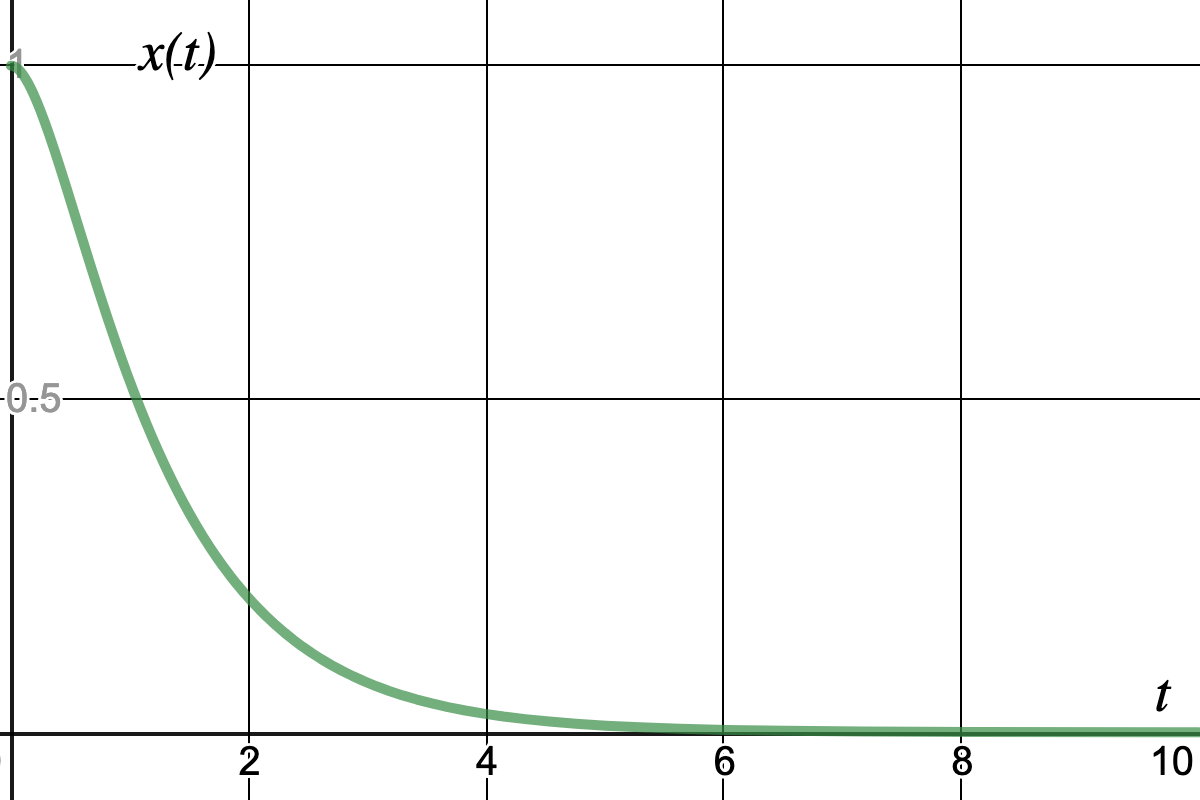
\includegraphics[width=.7\textwidth]{desmos-graph(19).png}
    \end{figure}
    \item The solution decays exponentially over time.  As $t\to \infty$ our solution approaches zero.
\end{enumerate}
\end{solution}

\newpage
\begin{problem}
Write down a homogeneous second-order linear differential equation where the system displays a decaying oscillation.
\end{problem}
\begin{solution}
Since our solution should oscillate and decay, we need some form of a ``spring" and some form of damping.  These terms show up respectively as $b$ and $c$ in the equation
\[
x''+bx'+cx=0.
\]
Now, also note that (aside from one special case of two of the same real roots), our general solution has the form
\[
x(t)=C_1 e^{\lambda_1 t}+C_2e^{\lambda_2 t}
\]
where $\lambda_1$ and $\lambda_2$ are roots to the characteristic polynomial
\[
\lambda^2+b\lambda + c =0.
\]
Now, the roots for the characteristic polynomial are
\[
\lambda = \frac{-b \pm \sqrt{b^2-4c}}{2}.
\]
\begin{itemize}
    \item To have oscillation, our roots must have an imaginary part and thus 
    \[
    b^2-4c<0.
    \]
    In other words, $b^2<4c.$
    \item To have a decaying solution, the real part of the roots must be negative. The real part of the roots will be $\frac{-b}{2}$ and thus we need
    \[
    \frac{-b}{2}<0.
    \]
\end{itemize}
Now, I'll choose $b=1$ and $c=1$ which satisfy both of these requirements. We then have
\[
x''+x'+x=0
\]
as our equation.

Note, we can also find the solution as the roots are then
\[
\lambda = \frac{-1\pm \sqrt{1-4}}{2}=\frac{-1}{2}\pm \frac{\sqrt{3}}{2}.
\]
Plugging this into the form for the general solution and we get
\[
x(t)=e^{-\frac{1}{2}t}\left(C_1 \sin\left(\frac{\sqrt{3}}{2}\right) + \cos\left(\frac{\sqrt{3}}{2}\right)\right)
\]
\end{solution}

\newpage
\begin{problem}
Consider the following differential equation:
\[
x''+2x'+x=3e^{-t}+2t.
\]
\begin{enumerate}[(a)]
    \item Find the homogeneous solution $x_H(t)$.
    \item Find the particular integral $x_P(t)$.
    \item Find the specific solution corresponding to the initial data $x(0)=0$, $x'(0)=0$.
\end{enumerate}
\end{problem}
\begin{solution}~
\begin{enumerate}[(a)]
    \item The roots to characteristic polynomial satisfy
    \[
    \lambda^2 + 2\lambda + 1 = 0
    \]
    which can be found by factoring
    \[
    (\lambda+1)^2=0,
    \]
    which gives us that $\lambda=-1$ is the only root.  Thus, this is the special case where our general solution looks slightly different.  We'll have
    \[
    x_h(t)=C_1e^{-t}+C_2te^{-t}.
    \]
    \item The right hand side has a $e^{-t}$ term which is already present in our $x_h$. In fact, this means we have to take $kt^2e^{-t}$ as a guess for this part of $x_p$. Then, we also have a $2t$ term, so our $x_p$ should be
    \[
    x_p =kt^2e^{-t}+ a_0 + a_1 t.
    \]
    Now we have to find the undetermined coefficients by plugging in and solving
    \begin{align*}
        x_p''+2x_p'+x_p&=3e^{-t}+2t\\
    2ke^{-t}-4kte^{-t}+kt^2e^{-t}+2(2kte^{-t}-kt^2e^{-t}+a_1)+kt^2e^{-t}a_1t+a_0&=3e^{-t}+2t
    \end{align*}
    which gives us that $k=\frac{3}{2}$, $a_1=2$, and $a_0=-4$. So 
    \[
    x_p(t)=\frac{3}{2}t^2e^{-t}+2t-4.
    \]
    \item Now, we take it that our solution is of the form
    \[
    x(t)=x_h+x_p= C_1e^{-t}+C_2te^{-t}+\frac{3}{2}t^2e^{-t}+2t-4.
    \]
    If we take
    \[
    0=x(0)=C_1-4
    \]
    then $C_1=4$, and
    \[
    0=x'(0)=-4+C_2+2
    \]
    so $C_2=2$. Thus, our specific solution is
    \[
    x(t)=(4+2t)e^{-t}+\frac{3}{2}t^2e^{-t}+2t-4.
    \]
    
\end{enumerate}
\end{solution}

\end{document}